% Chapter Template


\chapter{Method} % Main chapter title

\label{method} % Change X to a consecutive number; for referencing this chapter elsewhere, use \ref{ChapterX}

%learning_rate	0.001
%all_params	3,008,562
%trainable_params	3,003,930
%non_trainable_params	4,632
%layers	156
%training_time_1_epoch	85.43s
%description	Test adam optimizer on hrnet v7

\vspace*{\fill}
\begin{figure}[th]
    \centering
    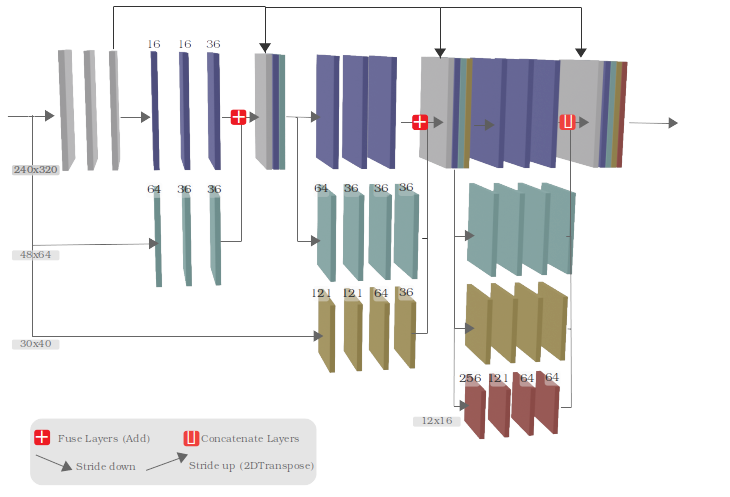
\includegraphics[width=150mm]{Figures/custom_hrnet_lines.png}
    \decoRule
    \caption[HRNetV3]{High-to-low representations network architecture}
    \label{fig:custom_hrnet}
\end{figure}
For our end-to-end keypoint recognition architecture we have created three modules to extract the background,
find the body parts in the image and detect the human joints or keypoints.
However, to extract the backround was not important for other keypoint recognition architectures such as
OpenPose~\cite{openpose} or VideoPose3D~\cite{videopose3d}, it is important in our architecture, since we wanted
this recognition architecture to be able to be used during practice, when there are multiple skaters on the ice,
but only track the focused skater.
With the body part detection module we altered the well established approach from OpenPose not to recognize vector
fields, which the joints connect,but the visible body parts.
We assume this method to work seamlessly, and estimate that this approach was not chosen before due to the missing
accurate labels for body part detection.
For the keypoint recognition module, we calculate the gaussian with a radius of three pixel and a standard deviation of
three.
In \autoref{fig:alena_step_labeled} we demonstrate an example frame labeld by our three modules
showing Alena Kostornaia, the 2020 European champion during her program.

\begin{figure}
    \centering
    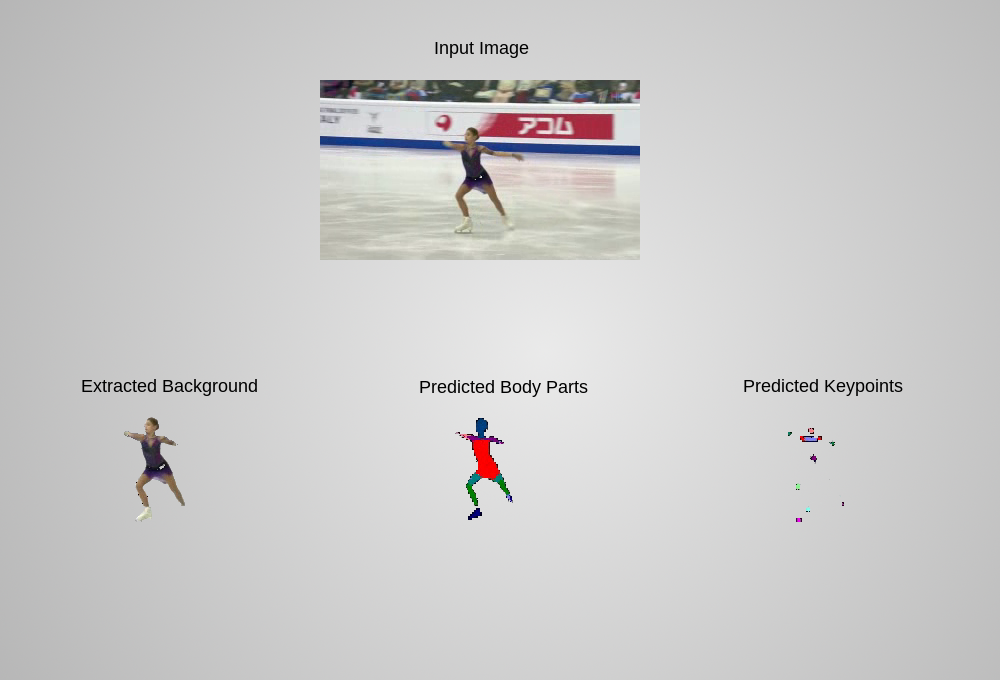
\includegraphics[width=130mm]{Figures/alena_step_labeled2.png}
    \decoRule
    \caption[Alena step]{Learned labels by the three modules: extracted background, human part detection and
    keypoint detection \textit{skater: Alena Kostornaia, 2020 European champion\cite{2020european}}}
    \label{fig:alena_step_labeled}
\end{figure}


All in all we have build a fully convolutional architecture with three networks, that all are based on high-to-low
representation learning. Our architecture consists of one input block $\mathcal{N}_I$  and three subsequent blocks
$\mathcal{N}_L$, $\mathcal{N}_M$,$\mathcal{N}_S$ and $\mathcal{N}_{XS}$.
These subsequent blocks combine feature maps with lower coarser representations with the original sized input image
feature maps and thus learn the features of the different levels equal to the HRNet strategy~\cite{HRNetv2, HRNetv1}.
\\\mbox{}\\
However, different from the HRNetV1 and HRNetV2 we do not use pooling to decrease or increase the size of the feature
maps. We decrease the feature maps with usual convolutions and accoring strides $\mathfrak{s}$ and kernel sizes
$\mathfrak{k}$, with $\mathfrak{s}=\mathfrak{k}$.
To increase the feature maps we use transposed convolutions with again $\mathfrak{s}=\mathfrak{k}$ according to the
strided down convolutions.
This allows the network to learn additional weights for the upward and downward convolutions and improve these level
exchange processes.
\\\mbox{}\\
Furthermore, we fuse the layer blocks in the first and second stage to combine the mentioned feature levels.
In the third stage however, we concatenate all feature levels to fully exploit the multi-resolution convolutions
as argued in HRNetV2~\cite{HRNetv2}.
\\\mbox{}\\
As visualized in~\ref{fig:custom_hrnet} we adjusted the amount of feature maps for the different blocks.
Moreover, in the first stage we use only three convolutional layers for one block int the other stages we use four layers
for the lower levels and only in $\mathcal{N}_L$ we use only three convolutional blocks throughout the network.
\\\mbox{}\\
Another adjustment is, that we use the input image as initial input for all our block levels but the $\mathcal{N}_{XS}$
block, wich uses the fused layers of all the other levels as input.
To every stage we add the input block $\mathcal{N}_I$.
\\\mbox{}\\
This network architecture resulted after several experiments and investigations of the estimated feature maps of the
different blocks and stages.
Every block is completed with batch normalization and a \textit{selu} activation functions.
The output of the network is predicted by a linear softmax activation function.
For the background-extraction and keypoint detection network we use mean-squared-error as loss functions and in the
human part detection network we use a custom loss function~\autoref{Experiments} to optimize the network weights.
In sum our network comprises 3,008,562 parameters of which 3,003,930 can be learned.
The amount of all layers for one network is 156.\\


% maybe put some images how the different modules did learn

%learning_rate	0.001
%all_params	3,008,562
%trainable_params	3,003,930
%non_trainable_params	4,632
%layers	156
%training_time_1_epoch	85.43s
%description	Test adam optimizer on hrnet v7


%----------------------------------------------------------------------------------------
%	SECTION 1
%----------------------------------------------------------------------------------------


%\section{Network Architecture}
%
%Lorem ipsum dolor sit amet, consectetur adipiscing elit. Aliquam ultricies lacinia euismod. Nam tempus risus in dolor
%rhoncus in interdum enim tincidunt. Donec vel nunc neque. In condimentum ullamcorper quam non consequat. Fusce
%sagittis tempor feugiat. Fusce magna erat, molestie eu convallis ut, tempus sed arcu. Quisque molestie, ante a
%tincidunt ullamcorper, sapien enim dignissim lacus, in semper nibh erat lobortis purus. Integer dapibus ligula ac
%risus convallis pellentesque.
%
%%-----------------------------------
%%	SUBSECTION 1
%%-----------------------------------
%
%\subsection{Body Part Detection Module}
%
%Nunc posuere quam at lectus tristique eu ultrices augue venenatis. Vestibulum ante ipsum primis in faucibus orci
%luctus et ultrices posuere cubilia Curae; Aliquam erat volutpat. Vivamus sodales tortor eget quam adipiscing in
%vulputate ante ullamcorper. Sed eros ante, lacinia et sollicitudin et, aliquam sit amet augue. In hac habitasse
%platea dictumst.
%
%%-----------------------------------
%%	SUBSECTION 2
%%-----------------------------------
%
%\subsection{Joint Detection Module}
%Morbi rutrum odio eget arcu adipiscing sodales. Aenean et purus a est pulvinar pellentesque. Cras in elit neque, quis
%varius elit. Phasellus fringilla, nibh eu tempus venenatis, dolor elit posuere quam, quis adipiscing urna leo nec
%orci. Sed nec nulla auctor odio aliquet consequat. Ut nec nulla in ante ullamcorper aliquam at sed dolor. Phasellus
%fermentum magna in augue gravida cursus. Cras sed pretium lorem. Pellentesque eget ornare odio. Proin accumsan, massa
%viverra cursus pharetra, ipsum nisi lobortis velit, a malesuada dolor lorem eu neque.

%----------------------------------------------------------------------------------------
%	SECTION 2
%----------------------------------------------------------------------------------------


\section{Training Performance (human parts)}
\begin{figure}
    \centering
    \includegraphics[width=130mm]{Figures/hp_accuracy_custom_hrnet_v3.png}
    \decoRule
    \caption[Alena step]{Learned labels by the three modules: extracted background, human part detection and
    keypoint detection \textit{skater: Alena Kostornaia, 2020 European champion\cite{2020european}}}
    \label{fig:hp_accuracy_hrnet_v3}
\end{figure}
\begin{figure}
    \centering
    \includegraphics[width=130mm]{Figures/hp_loss_custom_hrnet_v3.png}
    \decoRule
    \caption[Alena step]{Learned labels by the three modules: extracted background, human part detection and
    keypoint detection \textit{skater: Alena Kostornaia, 2020 European champion\cite{2020european}}}
    \label{fig:hp_loss_hrnet_v3}
\end{figure}

We trained the human parts module with the Adam optmizer for 5556 episodes, a batch size of 3 and 64 steps per epoch.
One training epoch took on average 85.43 seconds and took about 5.5 days.
For optimization we have build a custom loss function as explained in
\autoref{Experiments} to better deal with the class invariance of the occurring pixel labels.
The \autoref{fig:hp_accuracy_hrnet_v3} shows, that the accuracy of our network
\autoref{fig:hp_accuracy_hrnet_v3} rises very steep until the 500th episode and then flattens more and more until the last
episode, where the network reaches an excelent accuracy level of 0.99.
Furthermore, we devided our data in a distinct 90 percent train and 10 percent test dataset.
The figure shows equal trends for both datasets, which means the network did not overfit on the data.\

The loss function in \autoref{fig:hp_loss_hrnet_v3} shows equal opposite trends to the accuracy graph.
It steeply decreases until the 500th episode and then starts to flatten.
Again train and test dataset do not cross each other but show similar courses.

%----------------------------------------------------------------------------------------
%	SECTION 3
%----------------------------------------------------------------------------------------
\section{Inference Runtime Analysis}
The time to predict one frame of size 640x480 pixel takes about 0.3 seconds run on a Quad-Core Intel i7 CPU with 2.20 GHz,
a simple laptop cpu.
Predictions and training can run on simple hardware as the above mentioned cpu.
The training speed will increase if the minimum version of Cuda
3.5 is suported by the system, since then tensorflow 2 is able to run on the gpu instead of the cpu.
Due to the age of the named laptop cuda 3.0 was the highest to be supported.
Since recent developments targeting AI chips in the mobile world by the common companies Apple, Samsung or Huawei,
we are very confident that inference of our network does work as well on common sold mobile phones today~\cite{mobileAI}.
This sets apart our architecture from OpenPose, which we could not use for inference on the mentioned laptop.

%----------------------------------------------------------------------------------------
%	SECTION 4
%----------------------------------------------------------------------------------------
\section{Implementation Details}
We build our Network upon the high-level API TensorFlow 2 which is based on the Keras API~\cite{tensorflow2}.
Our training run on the AI server \textit{J.A.R.V.I.S.} provided by the Stuttgart Media University.
The server contains four Nvidia Titan Xp GPUs with 12 GB RAM and a i7 8-core CPU with 3.2 GHz.
We trained each experiment on a separate GPU. The training was conducted in docker containers using the TensorFlow
\textit{latest-devel-gpu}~\cite{tensorflowdocker} docker build.
The latest TensorFlow docker container did not support Python 3 at the time of this research, but only Python in version
2, which is why we had to use the before mentioned descendant.


